%%%%%%%%%%%%%%%%%%%%%%%%%%%%%%%%%
% 6CCS3PRJ Final Year Individual Project Report
% luke.day@kcl.ac.uk
%%%%%%%%%%%%%%%%%%%%%%%%%%%%%%%%%
\documentclass[11pt]{informatics-report}
\usepackage{color}
\usepackage[square,sort,comma,numbers]{natbib} %References

%%%%%%%%%%%%%%%%%%%%%%%%%%%%%%%%%
% Front Matter - project title, name, supervisor name and date
%%%%%%%%%%%%%%%%%%%%%%%%%%%%%%%%%
\title{6CCS3PRJ Final Year\\\vspace{0.2cm}[NC03]Automated Grading of SQL Tasks to Improve Student Learning}
\author{Vlad Stoica}
\studentID{1531350}
\supervisor{Criado Pacheco, Natalia}

\date{\today}

\abstractFile{FrontMatter/abstract.tex}
\ackFile{FrontMatter/acknowledgements.tex} %Remove line if you do not want acknowledgements

\begin{document}
\createFrontMatter
\onehalfspacing
\tableofcontents
\doublespacing

%%%%%%%%%%%%%%%%%%%%%%%%%%%%%%%%%
% Report Content
%%%%%%%%%%%%%%%%%%%%%%%%%%%%%%%%%
% You can write each chapter directly here or in a separate .tex file and use the include command.

\chapter{Introduction}
This is one of the most important components of the report. It should begin with a clear statement of what the project is about so that the nature and scope of the project can be understood by a lay reader. It should summarise everything that you set out to achieve, provide a clear summary of the project's background and relevance to other work, and give pointers to the remaining sections of the report, which will contain the bulk of the technical material.

\section{Report Structure}

\chapter{Background}
The background should set the project into context by motivating the subject matter and relating it to existing published work. The background will include a critical evaluation of the existing literature in the area in which your project work is based and should lead the reader to understand how your work is motivated by and related to existing work.

\section{Section Heading}
% \chapter{Report Body}
The central part of the report usually consists of three or four chapters detailing the technical work undertaken during the project. {\bf{\textcolor{red}{The structure of these chapters is highly project dependent}}}. They can reflect the chronological development of the project, e.g. design, implementation, experimentation, optimisation, evaluation, etc (although this is not always the best approach). However you choose to structure this part of the report, you should make it clear how you arrived at your chosen approach in preference to other alternatives. In terms of the software that you produce, you should describe and justify the design of your programs at some high level, e.g. using OMT, Z, VDL, etc., and you should document any interesting problems with, or features of, your implementation. Integration and testing are also important to discuss in some cases. You may include fragments of your source code in the main body of the report to illustrate points; the full source code is included in an appendix to your written report.

\section{Section Heading}

\subsection{Subsection Heading}
% \chapter{Design \& Specification}

\section{Section Heading}
% \chapter{Implementation}

\section{Section Heading}

% \chapter{Legal, Social, Ethical and Professional Issues}
Your report should include a chapter with a reasoned discussion about legal, social ethical and professional issues within the context of your project problem. You should also demonstrate that you are aware of the regulations governing your project area and the Code of Conduct \& Code of Good Practice issued by the British Computer Society, and that you have applied their principles, where appropriate, as you carried out your project.

\section{Section Heading}

% \chapter{Results/Evaluation}

\section{Software Testing}

\section{Section Heading}

% \chapter{Conclusion and Future Work}

The project's conclusions should list the key things that have been learnt as a consequence of engaging in your project work. For example, ``The use of overloading in C++ provides a very elegant mechanism for transparent parallelisation of sequential programs'', or ``The overheads of linear-time n-body algorithms makes them computationally less efficient than $O(n \log n)$ algorithms for systems with less than 100000 particles''. Avoid tedious personal reflections like ``I learned a lot about C++ programming...'', or ``Simulating colliding galaxies can be real fun...''. It is common to finish the report by listing ways in which the project can be taken further. This might, for example, be a plan for turning a piece of software or hardware into a marketable product, or a set of ideas for possibly turning your project into an MPhil or PhD.

%%%%%%%%%%%%%%%%%%%%%%%%%%%%%%%%%
% References
%%%%%%%%%%%%%%%%%%%%%%%%%%%%%%%%%
\bibliographystyle{plain}
\bibliography{references}
\addcontentsline{toc}{section}{Bibliography}

%%%%%%%%%%%%%%%%%%%%%%%%%%%%%%%%%
% Appendices
%%%%%%%%%%%%%%%%%%%%%%%%%%%%%%%%%
\appendix
% \include{Appendices/appendix}
% \chapter{User Guide}

\section{Getting the web application running}
\subsection{Installation}
One must only install the web application, as the library is automatically pulled when installing the requirements.

\begin{enumerate}
    \item Install dependencies: \texttt{\$ bundle install}
    \item Update database configuration:
    \begin{enumerate}
        \item Update \texttt{config/database.yml} with the MySQL details for the web application
        \item Update \texttt{config/initializers/assesor.rb} with the MySQL details for the web application
    \end{enumerate}
    \item Create web application database: \texttt{\$ bin/rake db:setup}
    \item Run database migrations: \texttt{\$ bin/rake db:migrate}
\end{enumerate}

\subsection{Starting the server}

The web application can be started using the command \texttt{bin/rails server}. The web application will be accessible on \texttt{localhost:3000}.

There are two defaults users created:
\begin{enumerate}
    \item Admin user:
    \begin{enumerate}
        \item Email: admin@example.com
        \item Password: test123
    \end{enumerate}
    \item Student user:
    \begin{enumerate}
        \item Email: student@example.com
        \item Password: test123
    \end{enumerate}
\end{enumerate}

\section{User management}
\Oldsubsection{Authentication}
A user must be authenticated at all time to access the application's functionality. Authentication is done on the path \texttt{/users/sign\_in}. A user will be automatically redirected to this page if he is not logged in. If a user uses a wrong email or password combination, he will see an error. The log in page is presented in figure \ref{fig:app:authentication}.

\begin{figure}[ht]
    \centering
    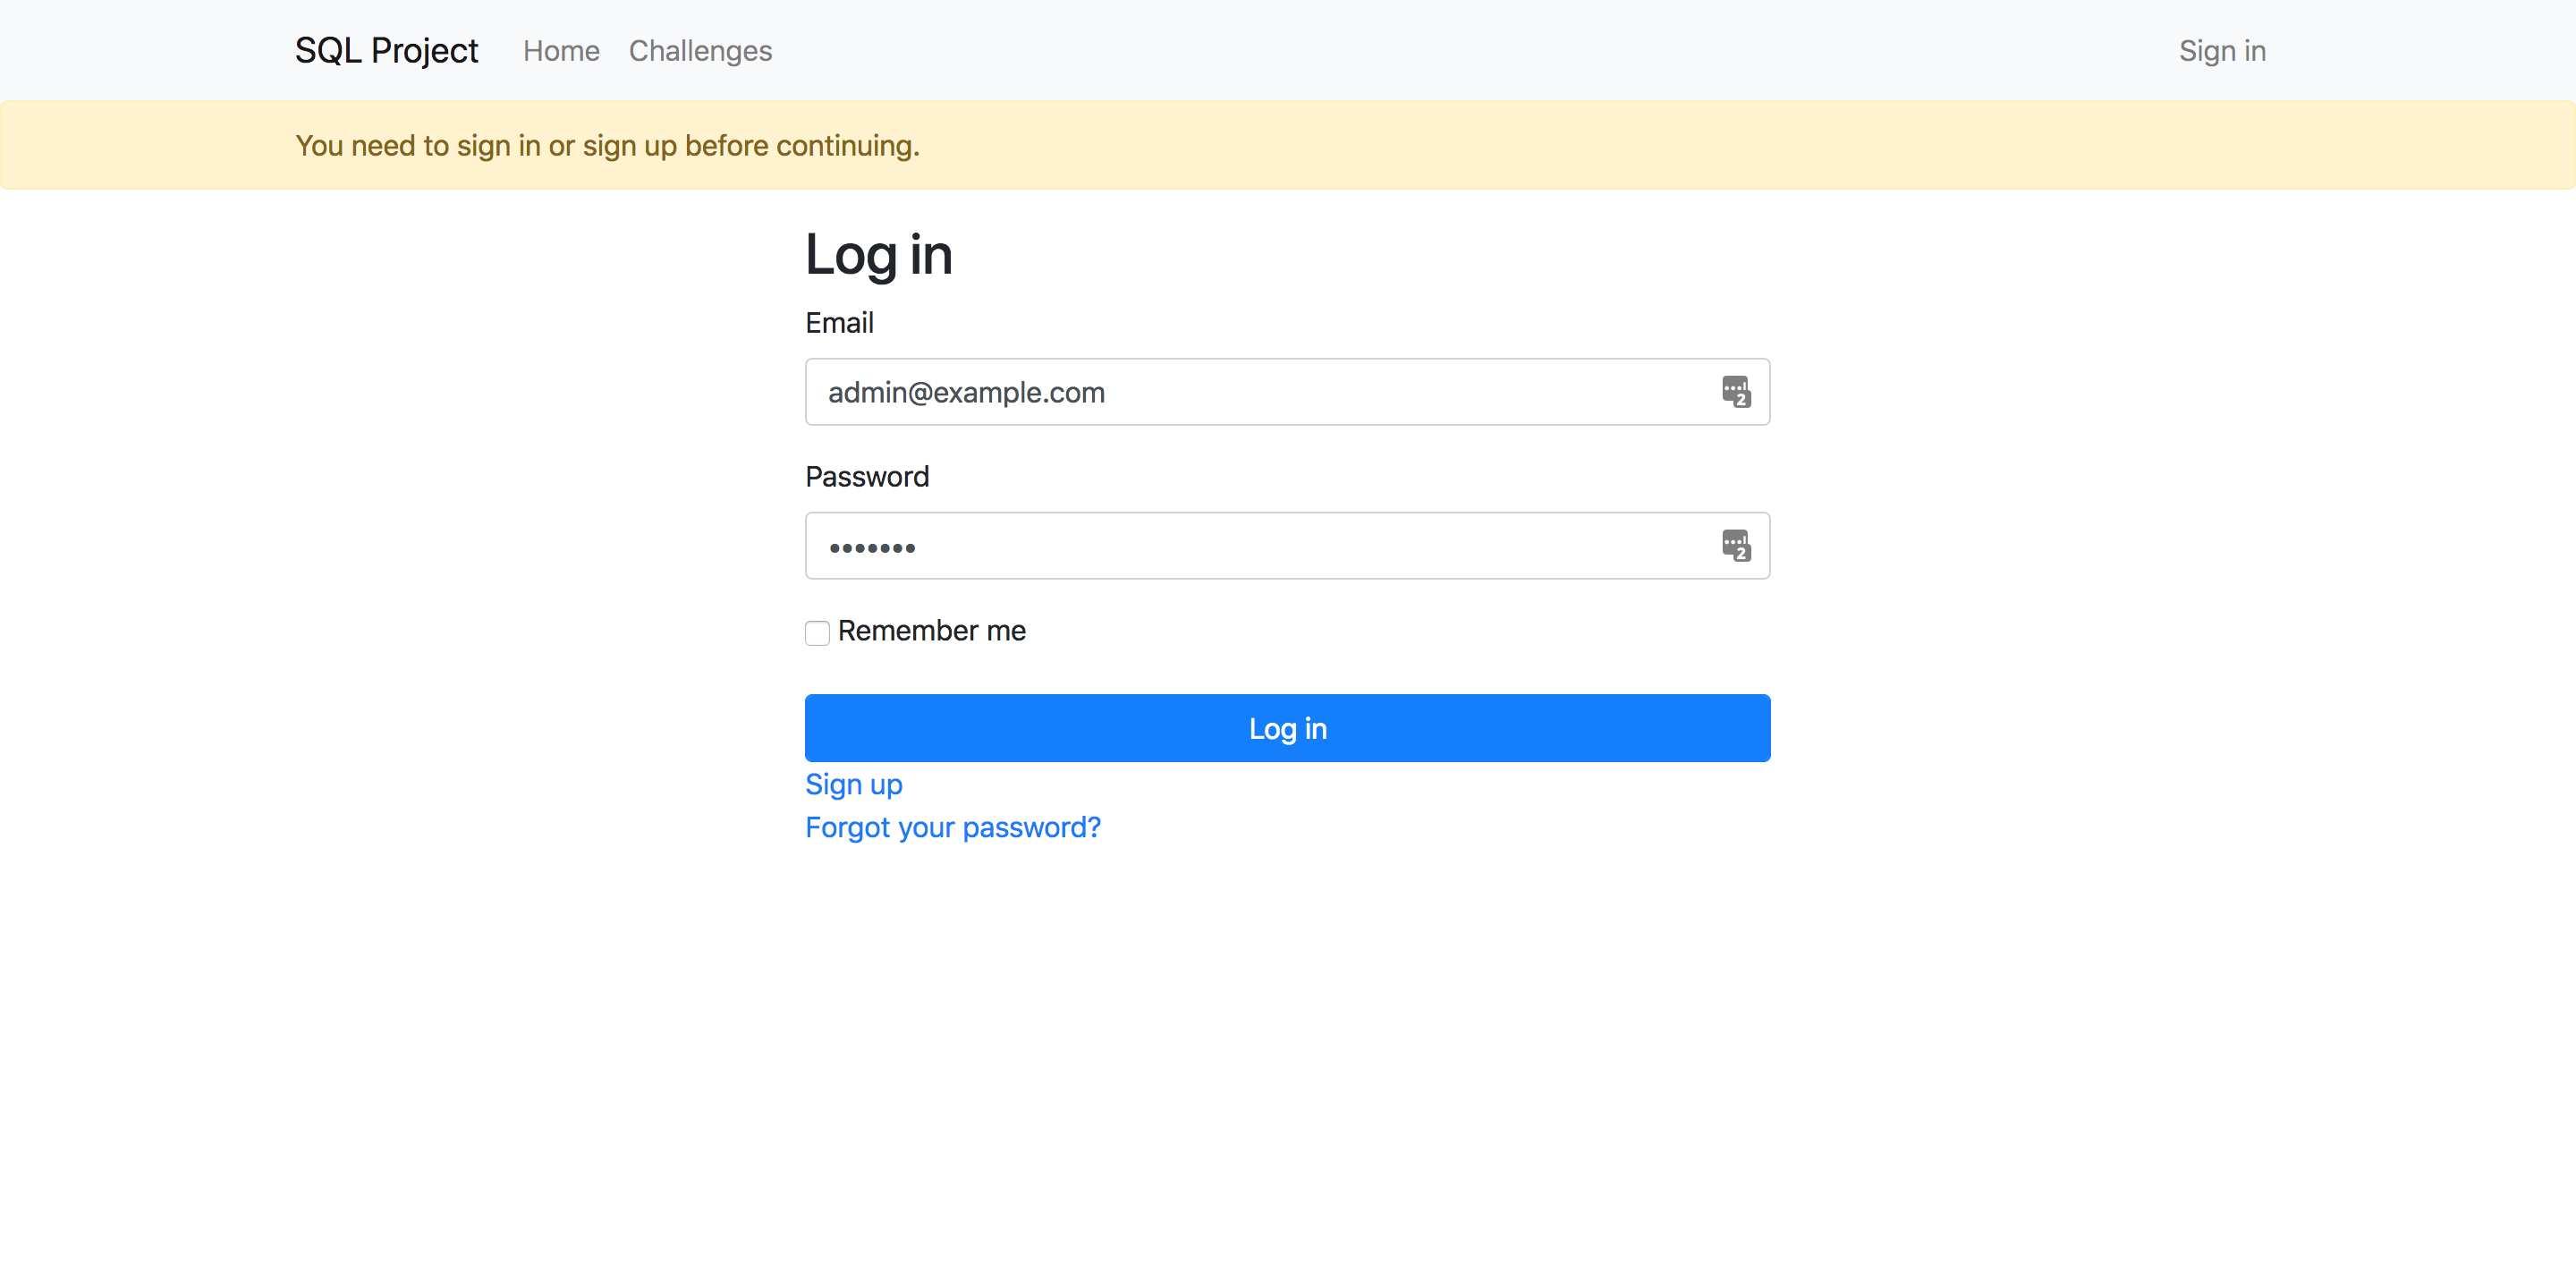
\includegraphics[width=\textwidth/4*3]{Appendices/authentication.png}
    \caption{Authentication screen}
    \label{fig:app:authentication}
\end{figure}

\Oldsubsection{Creating new user}
A new user can be created on the web application on path \texttt{/users/sign\_up} or by clicking the sing up button from the login page. Users are automatically marked as students. If a user uses a wrong email or password combination, he will see an error. An example of the sign-up page with errors is presented in figure \ref{fig:app:newuser}.

\begin{figure}[ht]
    \centering
    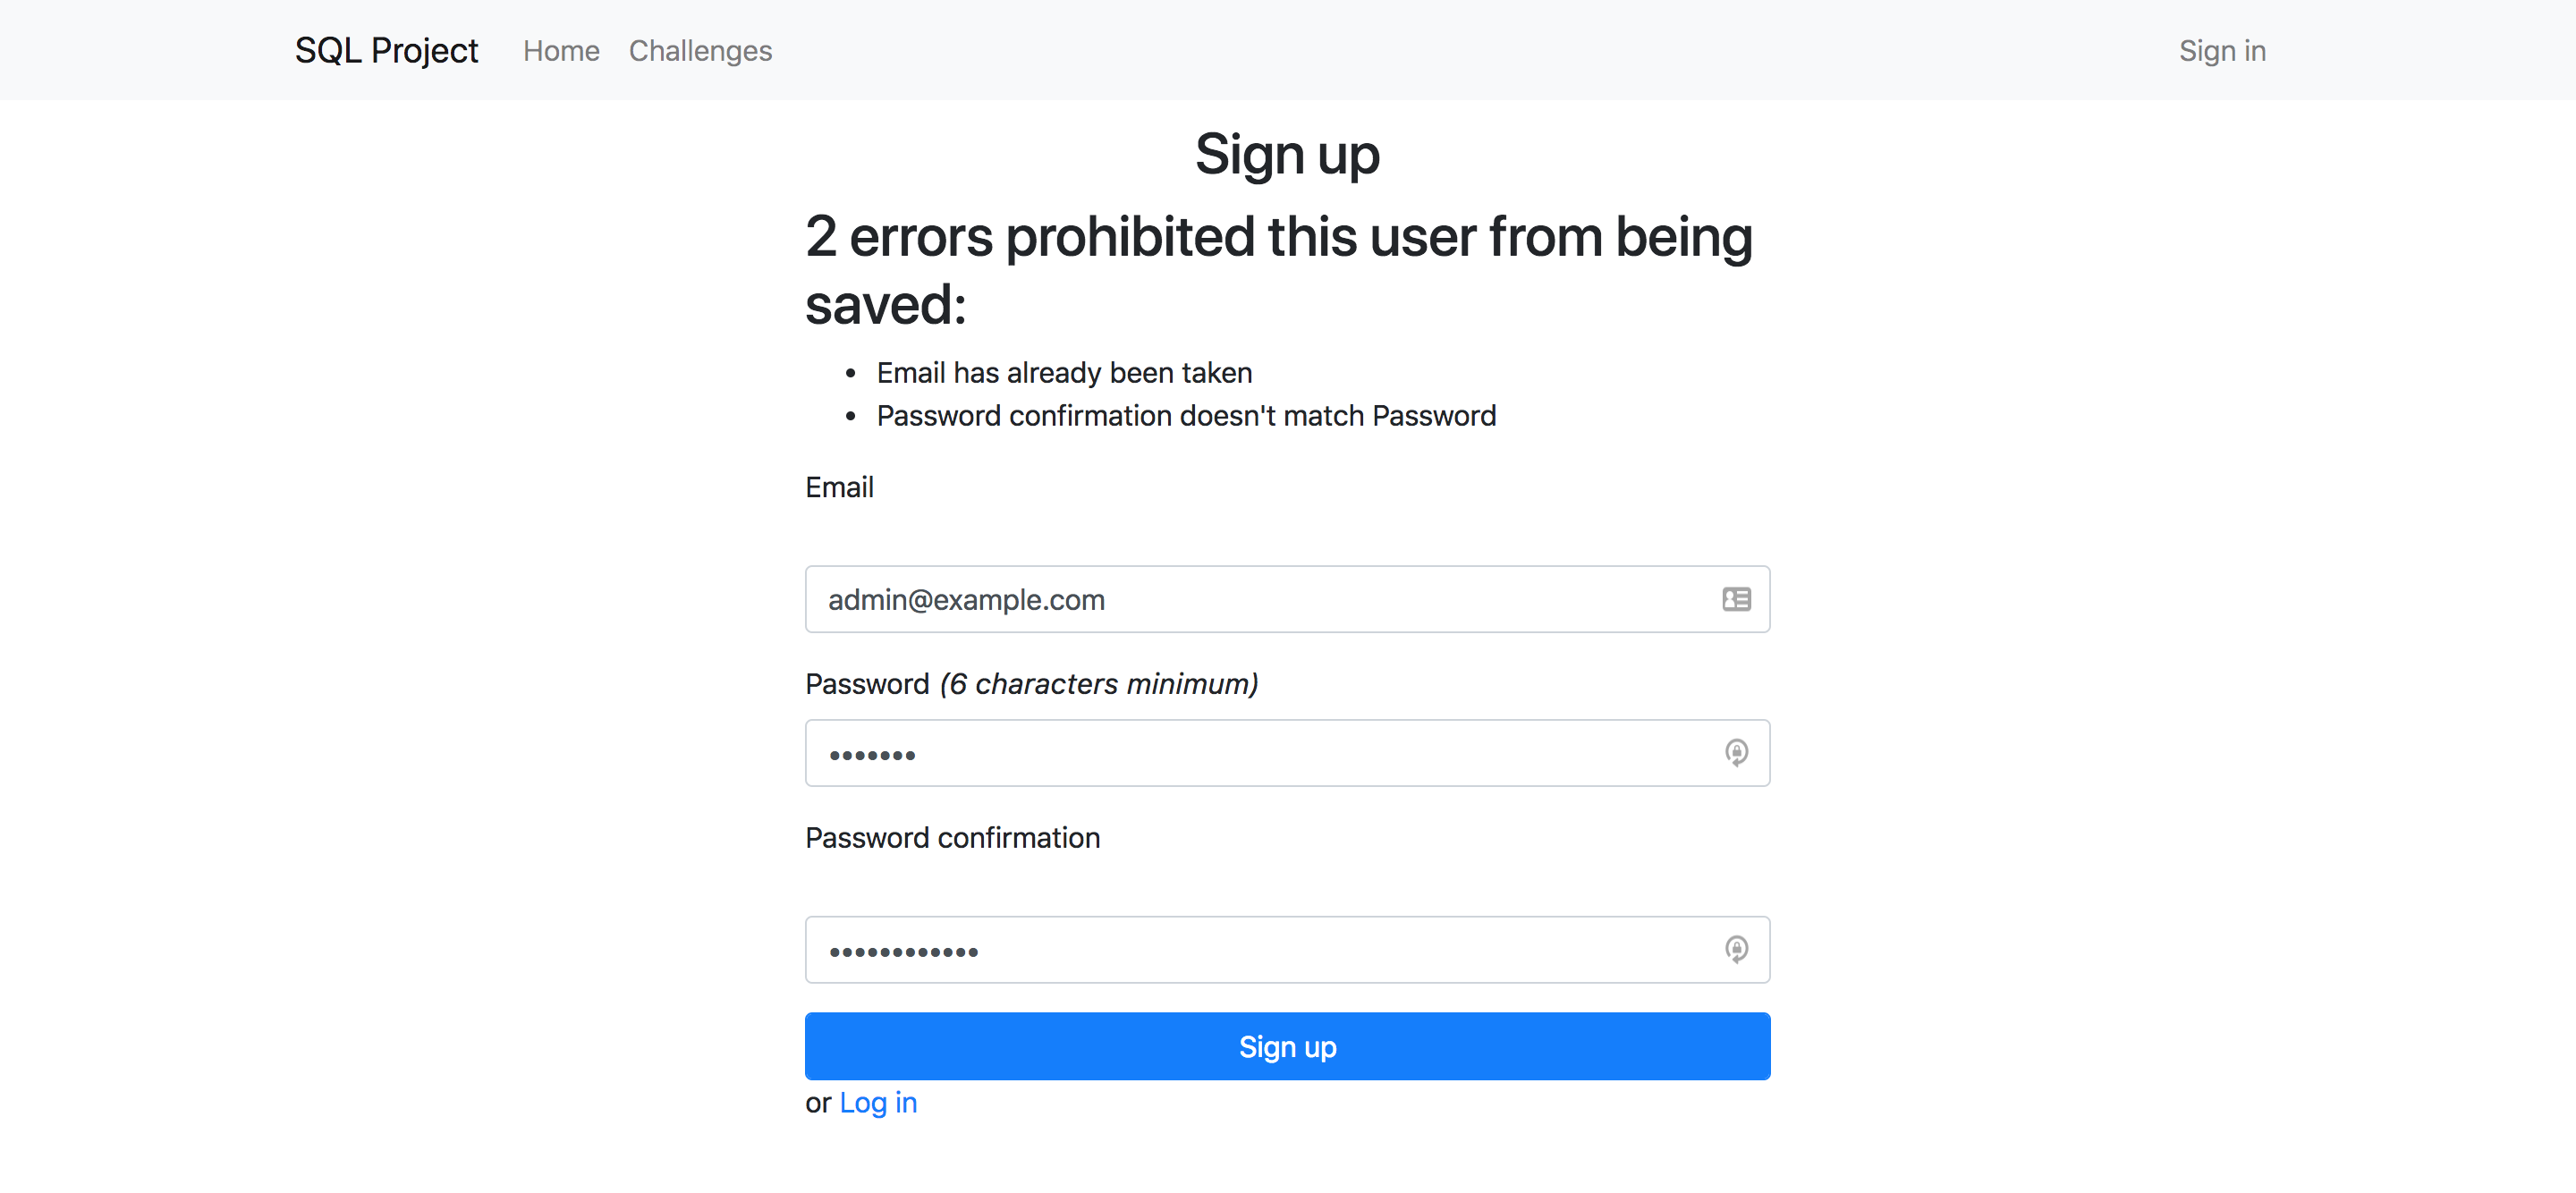
\includegraphics[width=\textwidth/4*3]{Appendices/signup.png}
    \caption{Sign-up screen}
    \label{fig:app:newuser}
\end{figure}

\Oldsubsection{Editing user details}
A user can change his details (email and password) on \texttt{/users/edit} or by clicking the Edit Profile in the navigation bar. The navigation bar link is presented in figure \ref{fig:app:editusernavbar} On this page, he can also delete his account. A photo of the page is included in figure \ref{fig:app:edituser}.

\begin{figure}[ht]
    \centering
    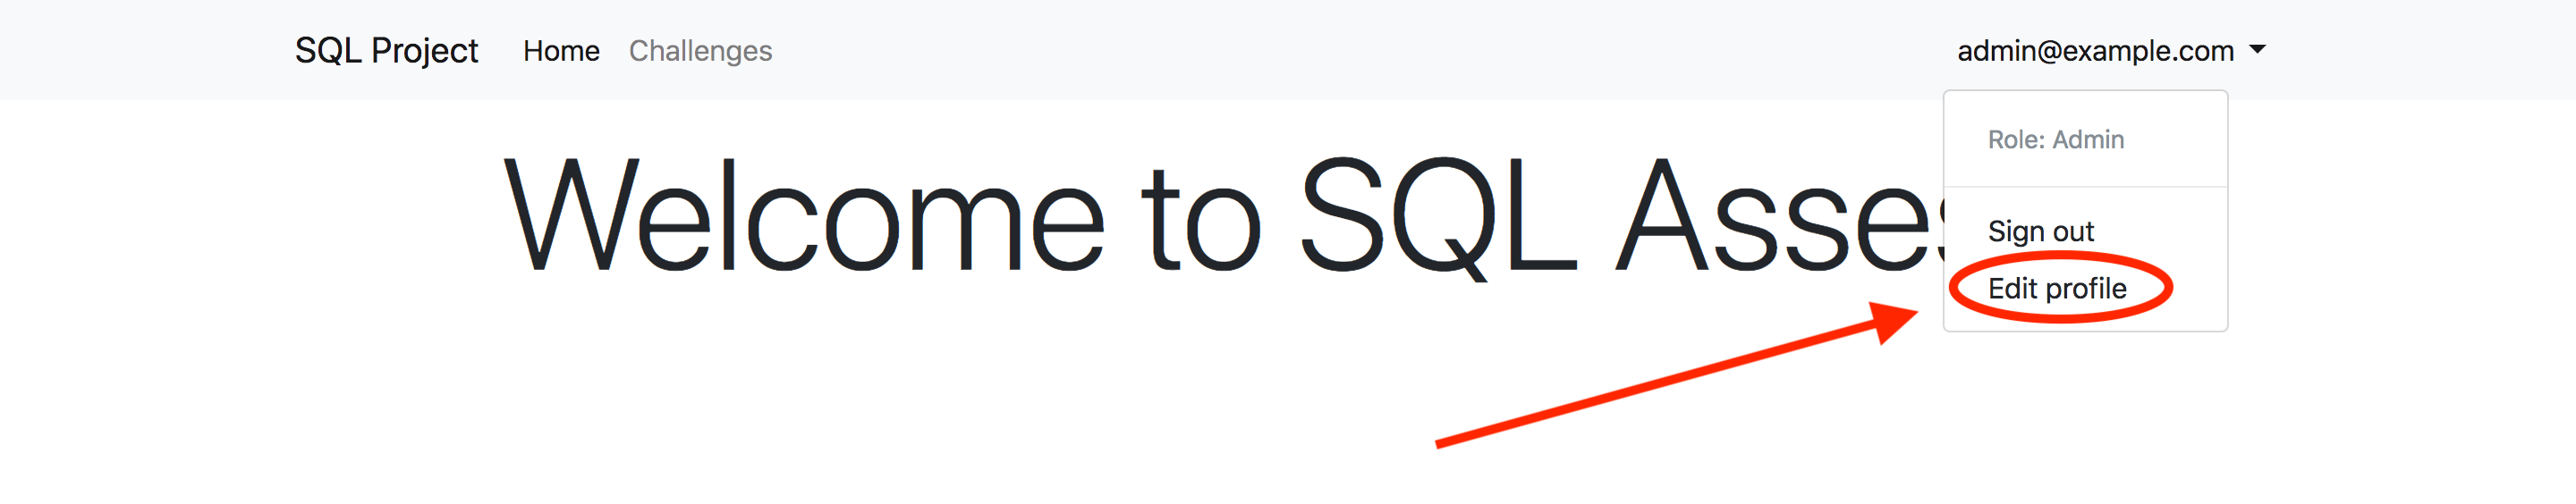
\includegraphics[width=\textwidth/4*3]{Appendices/editlinknavbar.png}
    \caption{Navigation bar link for edit user}
    \label{fig:app:editusernavbar}
\end{figure}

\begin{figure}[ht]
    \centering
    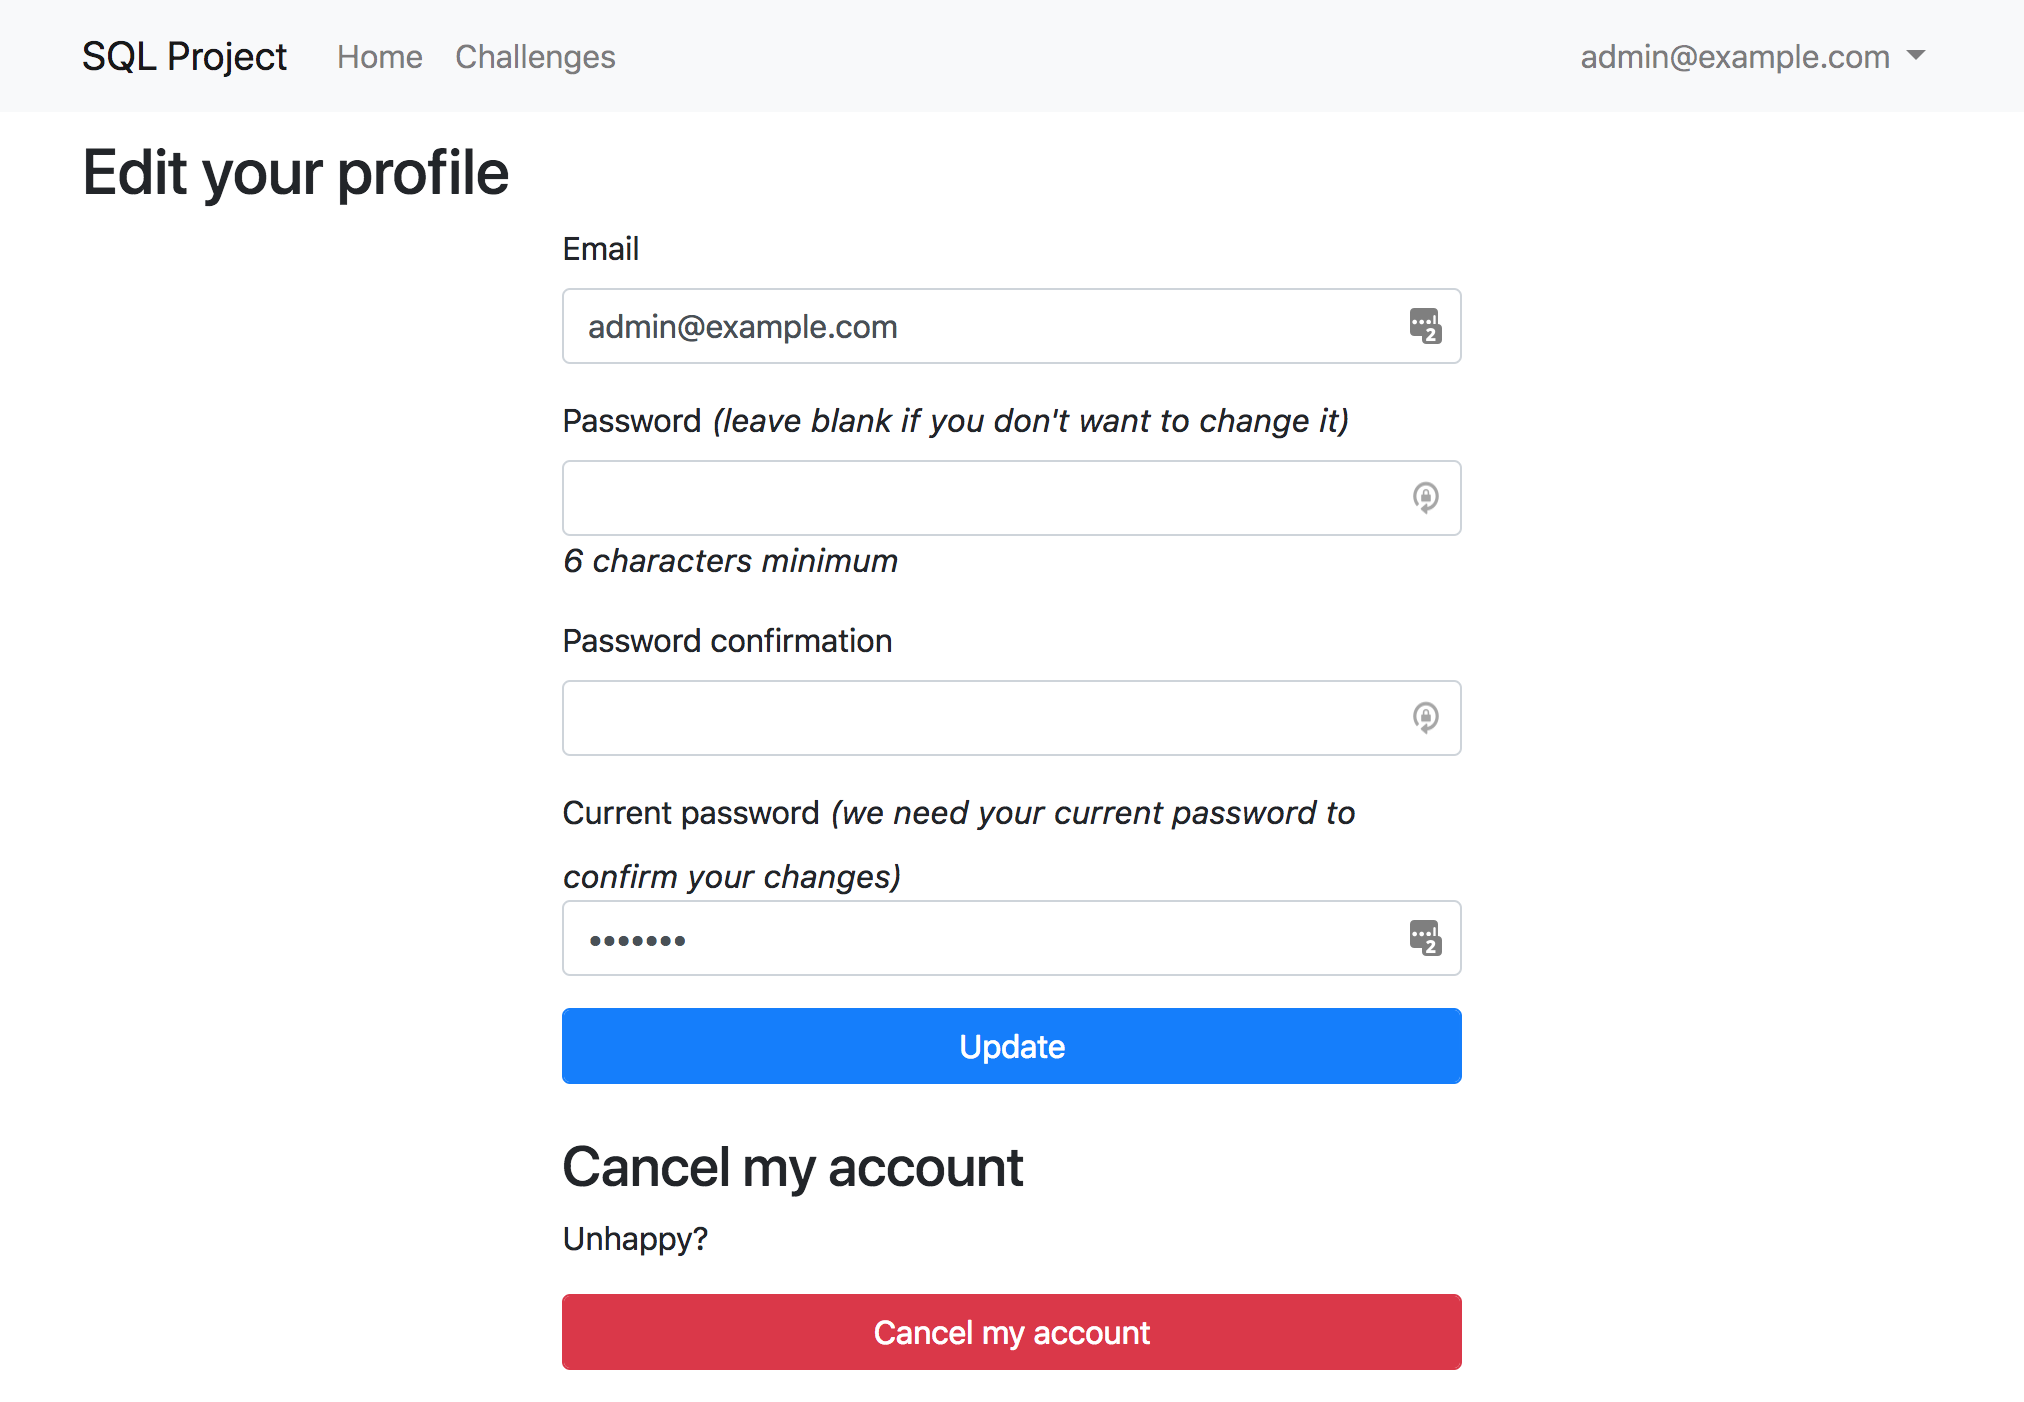
\includegraphics[width=\textwidth/4*3]{Appendices/edituser.png}
    \caption{Edit user page}
    \label{fig:app:edituser}
\end{figure}

\Oldsubsection{Sign-out}
Signing out is done from the navigation bar. Figure \ref{fig:app:signout} presents the location of the button.

\begin{figure}[ht]
    \centering
    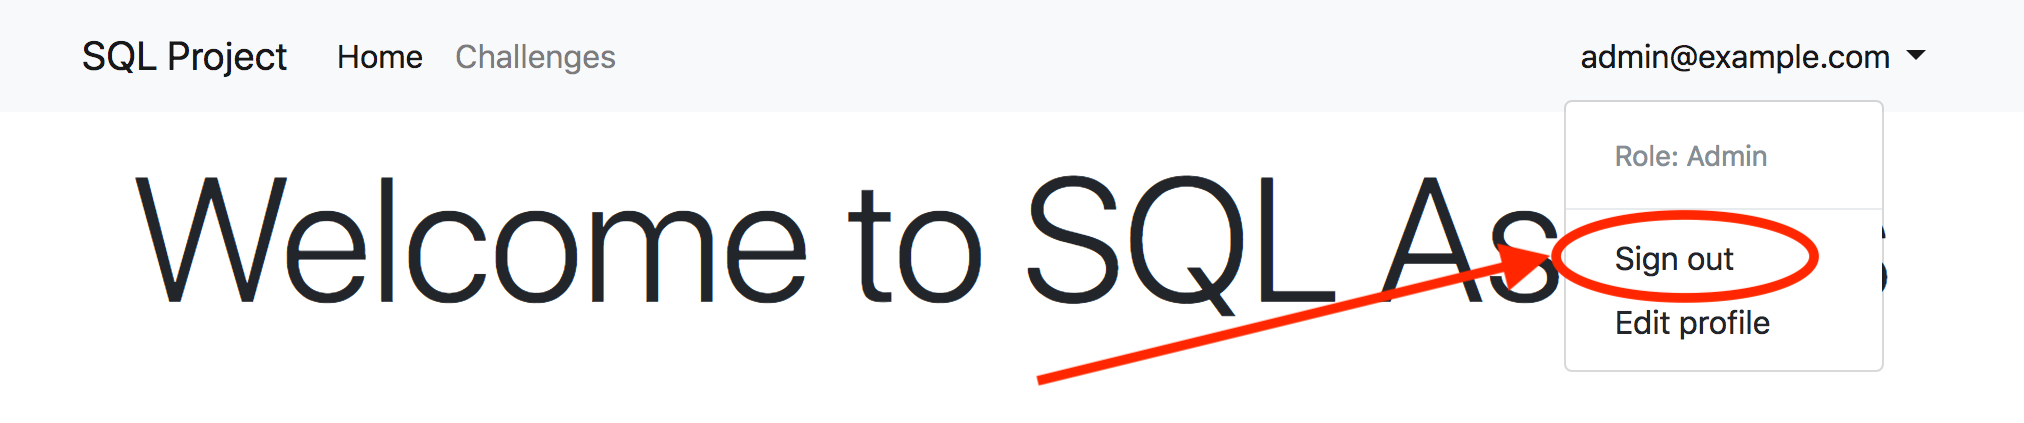
\includegraphics[width=\textwidth/4*3]{Appendices/signout.png}
    \caption{Sign out button}
    \label{fig:app:signout}
\end{figure}

\section{Challenge management}
To create a challenge, the current user must be an admin. To create a challenge, one must go to \texttt{/challenges/new}, or click \textit{Challenges} in the navigation bar, and then click \textit{Create new Challenge} button. The screen is presented in figure \ref{fig:app:new_challenge}.

The new challenge page requires 5 pieces of information:
\begin{enumerate}
    \item A title for the challenge
    \item The content or the challenge - or the body of the challenge
    \item SQL query for schema creation
    \item SQL query for data insertion
    \item The correct SQL query for the challenge
\end{enumerate}

The input for the SQL fields is a code editor that provides code syntax highlighting.

Any errors that might be encountered are shown to the user.
\begin{figure}[ht]
    \centering
    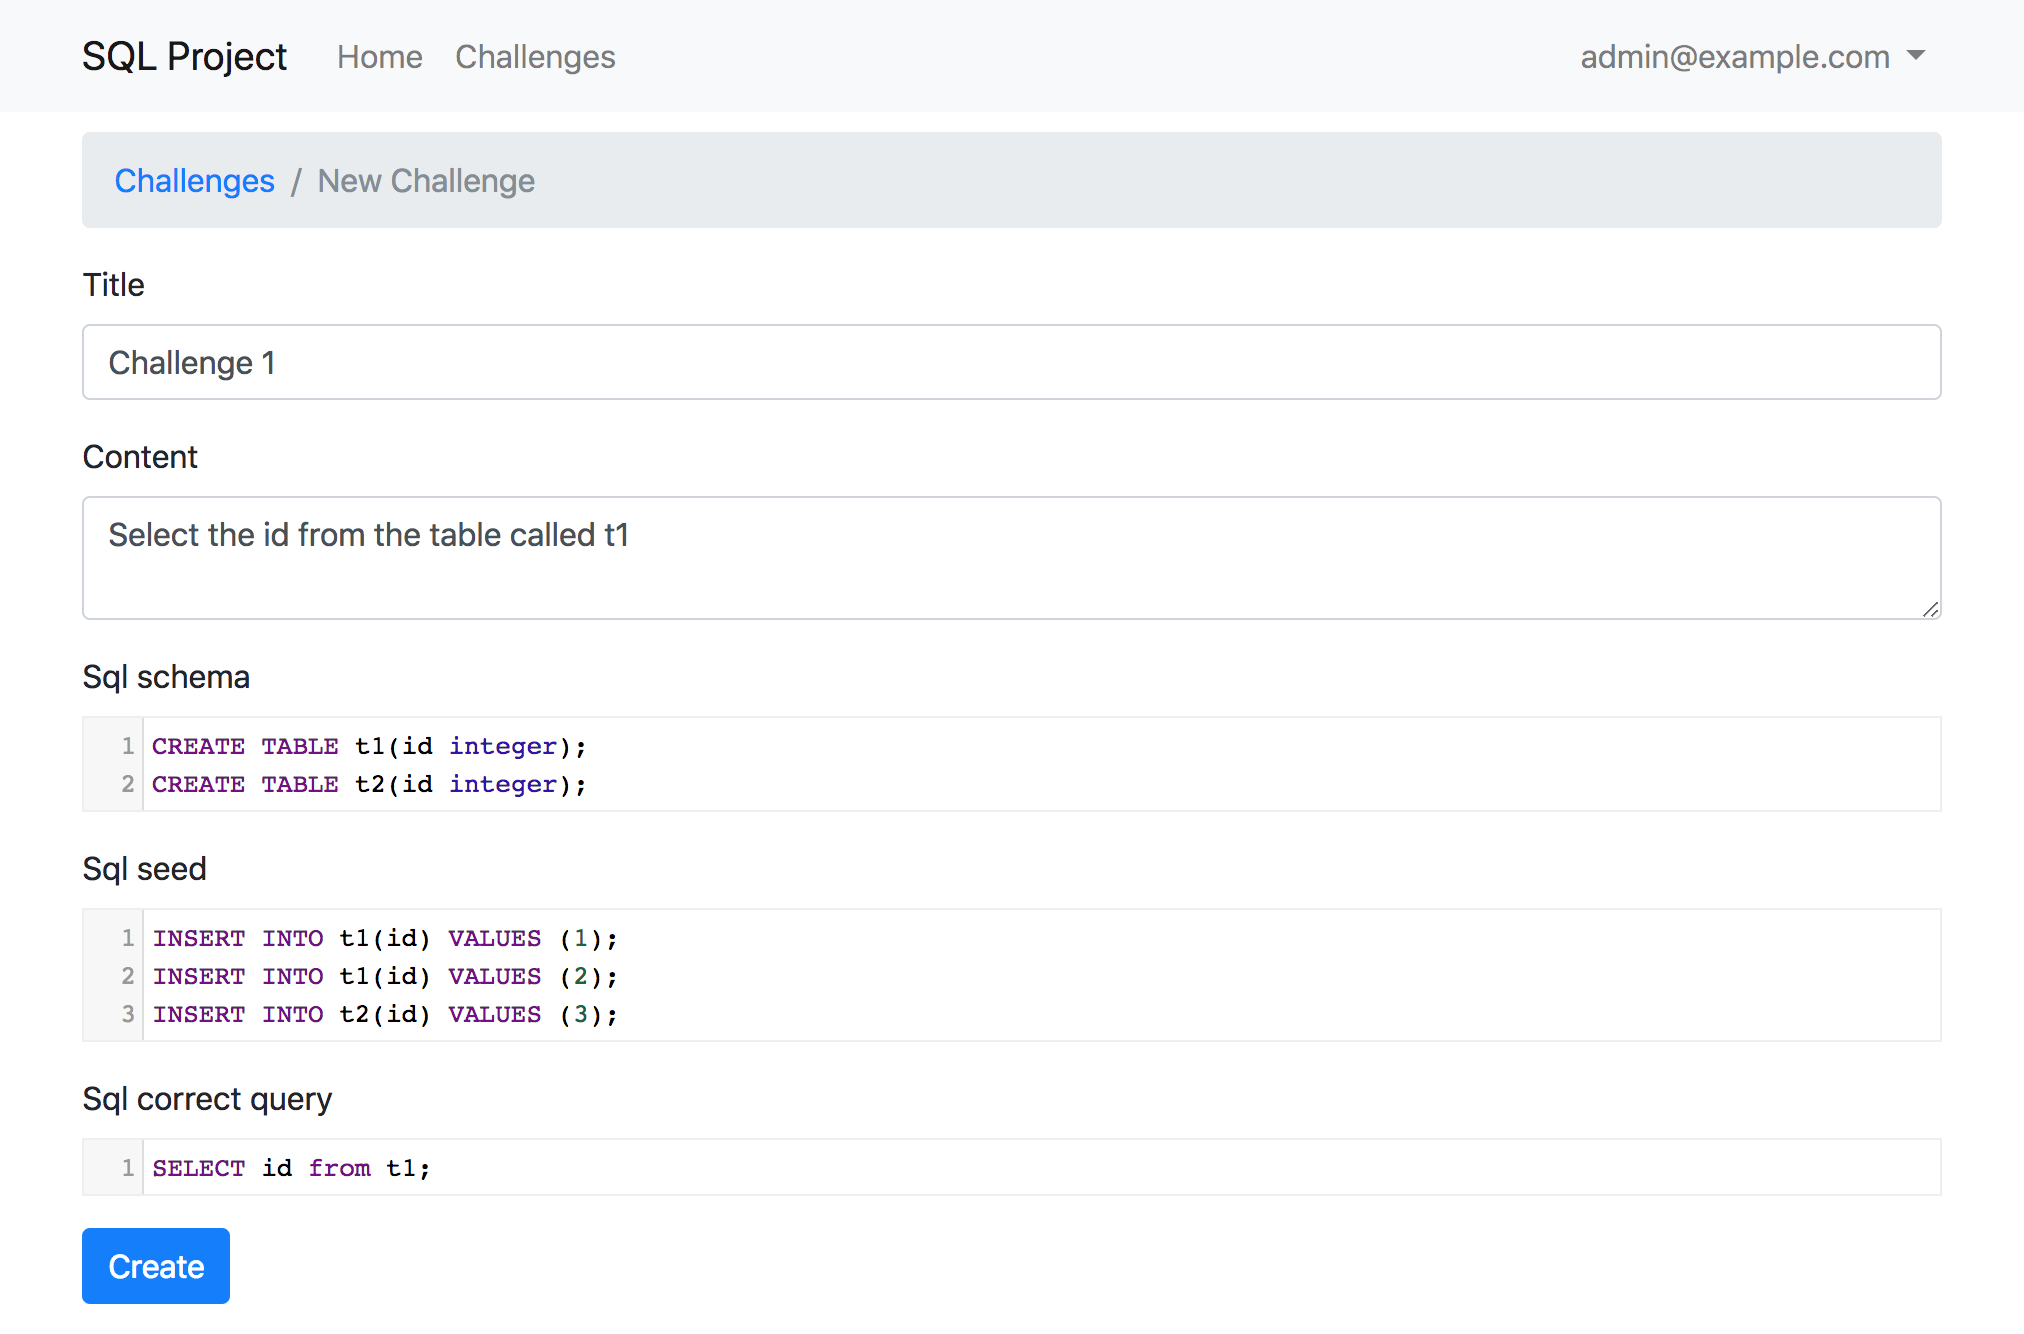
\includegraphics[width=\textwidth/4*3]{Appendices/new_challenge.png}
    \caption{New challenge form}
    \label{fig:app:new_challenge}
\end{figure}

Once the challenge has been saved, the user is redirect to the challenge page which contains all the details about the challenge (schema and existing fields). A screen-shot of the page is show in figure \ref{fig:app:challengeadmin}.

\begin{figure}[ht]
    \centering
    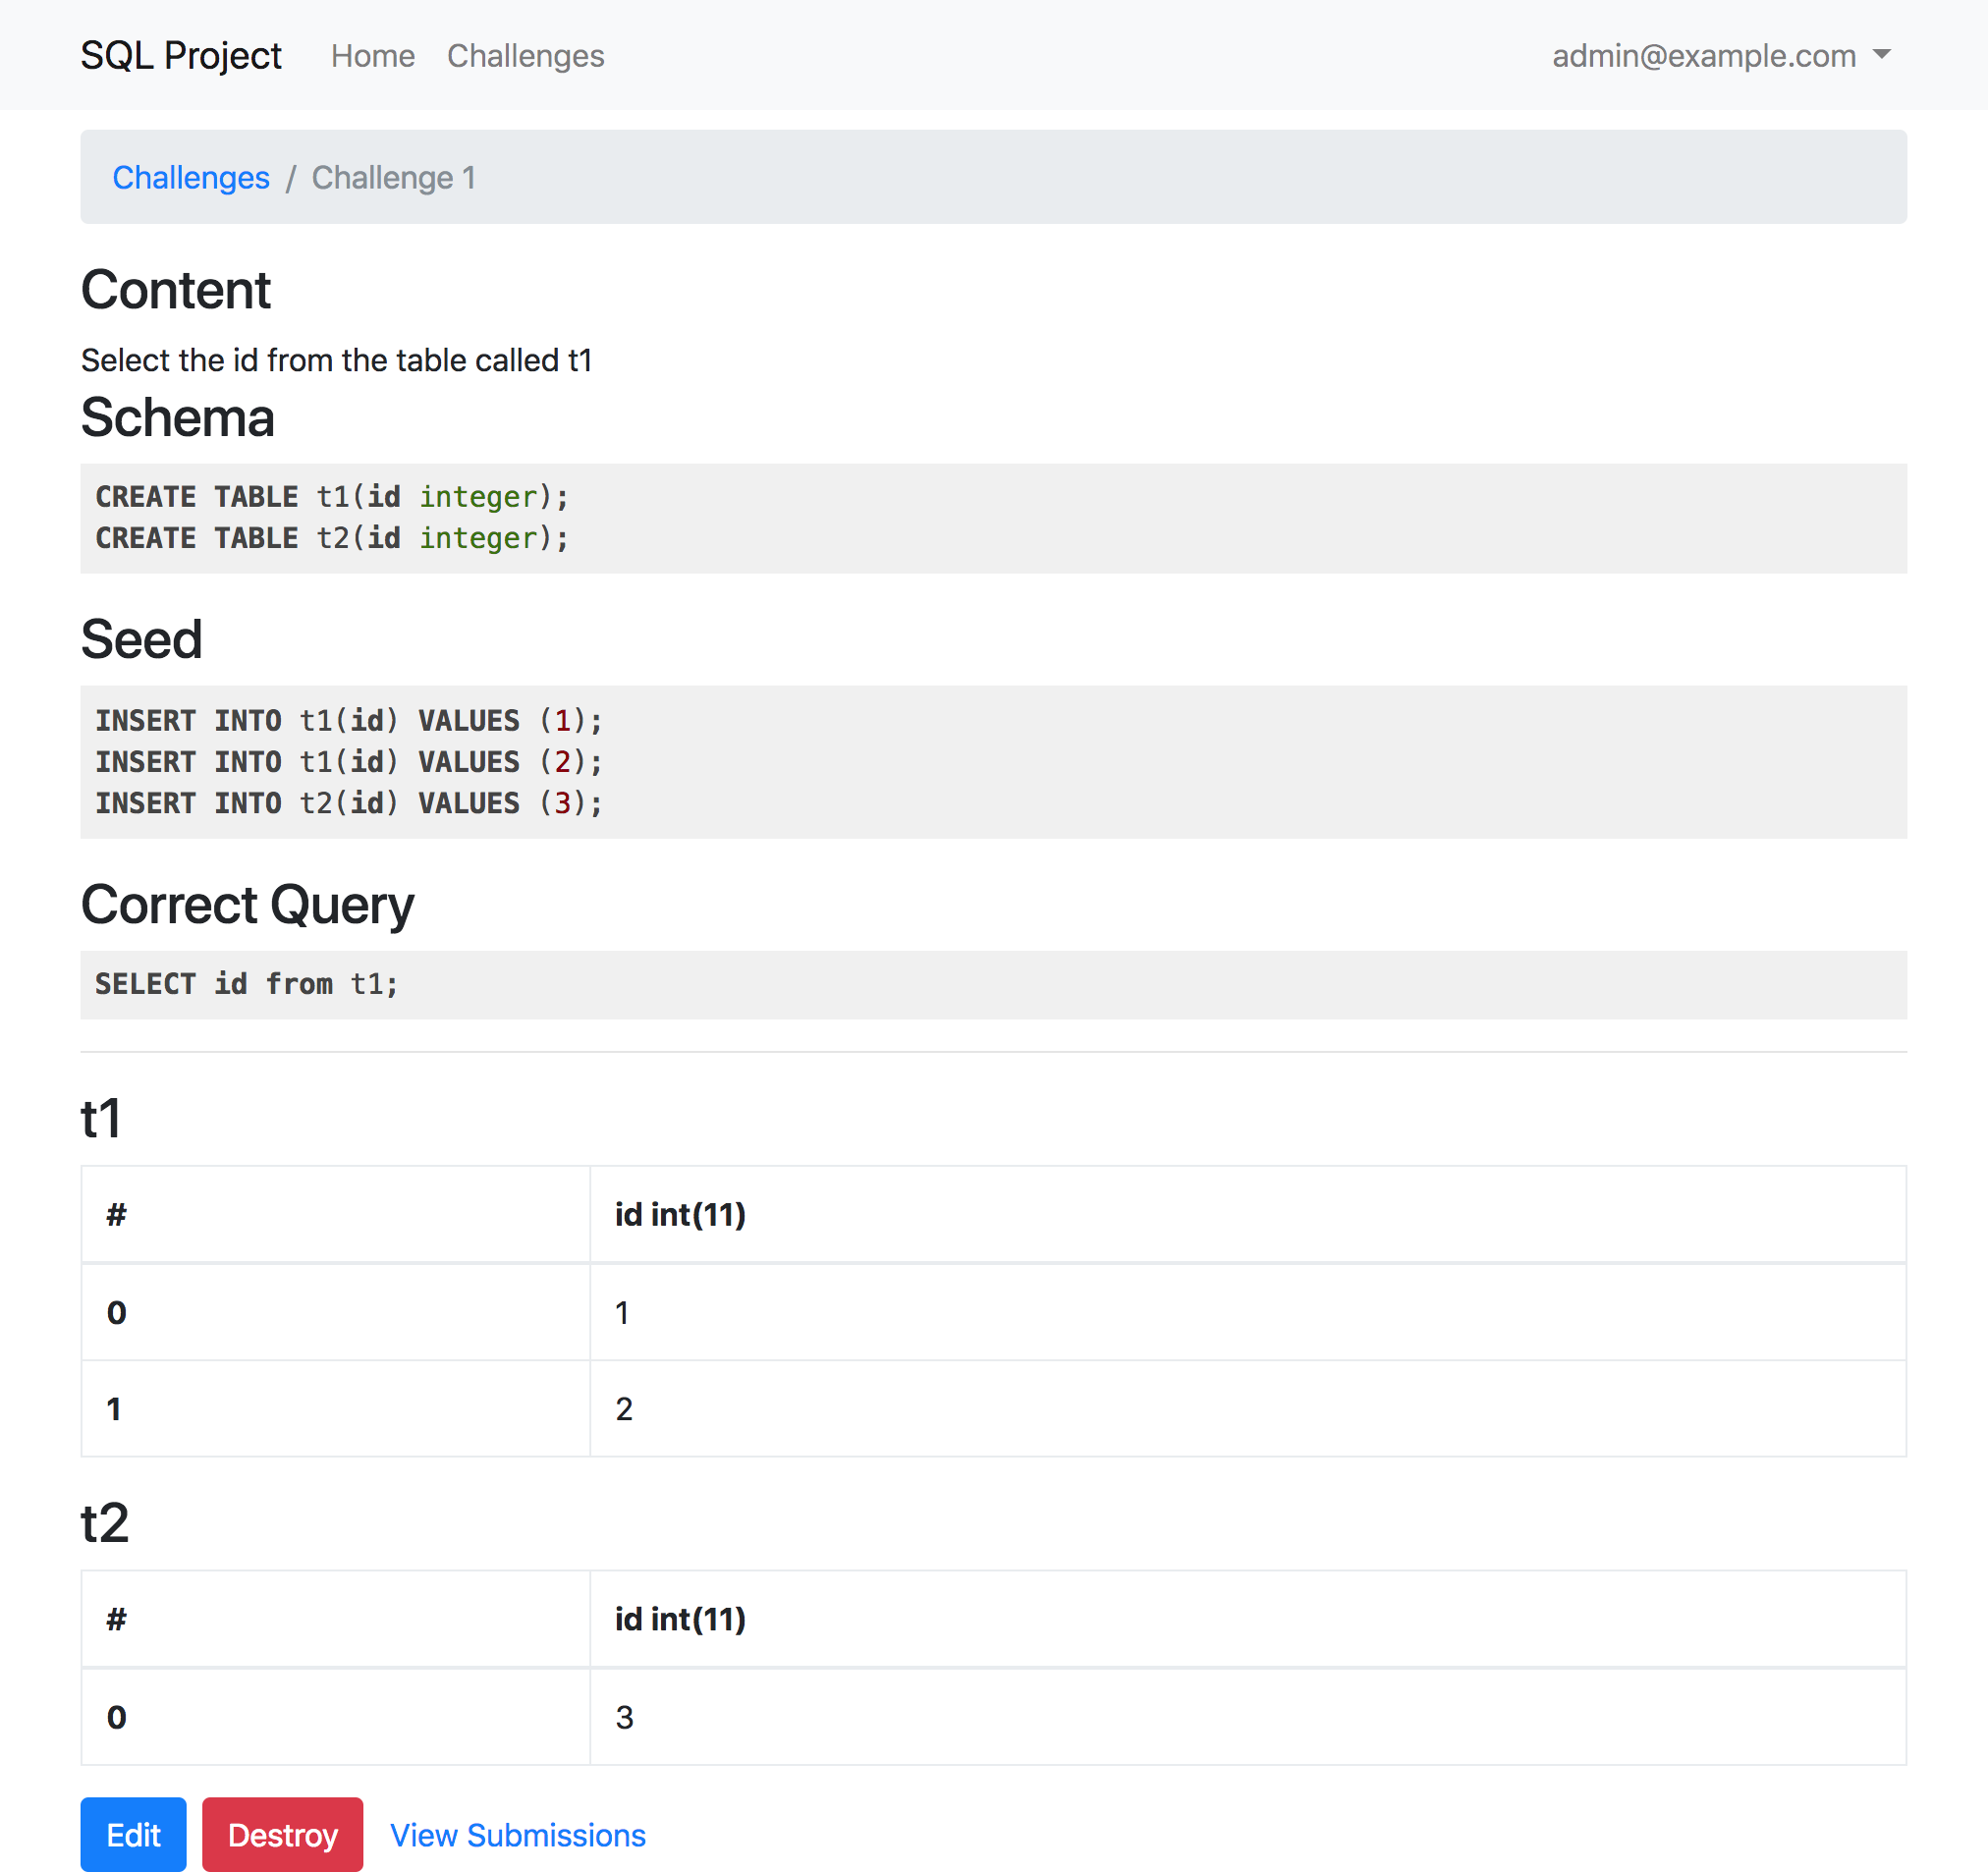
\includegraphics[width=\textwidth/4*3]{Appendices/adminchallenge.png}
    \caption{Admin's view of a new challenge}
    \label{fig:app:challengeadmin}
\end{figure}

An admin can then edit any challenge by clicking the edit button at the bottom of the page \ref{fig:app:challengeadmin}. The edit page is very similar to the creation form (\ref{fig:app:new_challenge}).

An admin can also delete a challenge by clicking the Destroy button at the bottom of the page \ref{fig:app:challengeadmin}.

\section{Submissions: student's view}

A student can submit a solution by first going to the \textit{New submission page}. To go to that page, he first needs to visit the challenges page (from the navigation bar), and then click the \textit{New submission} link for the desired challenge. The instructions are presented in figure \ref{fig:app:new_submission}.

\begin{figure}[ht]
    \centering
    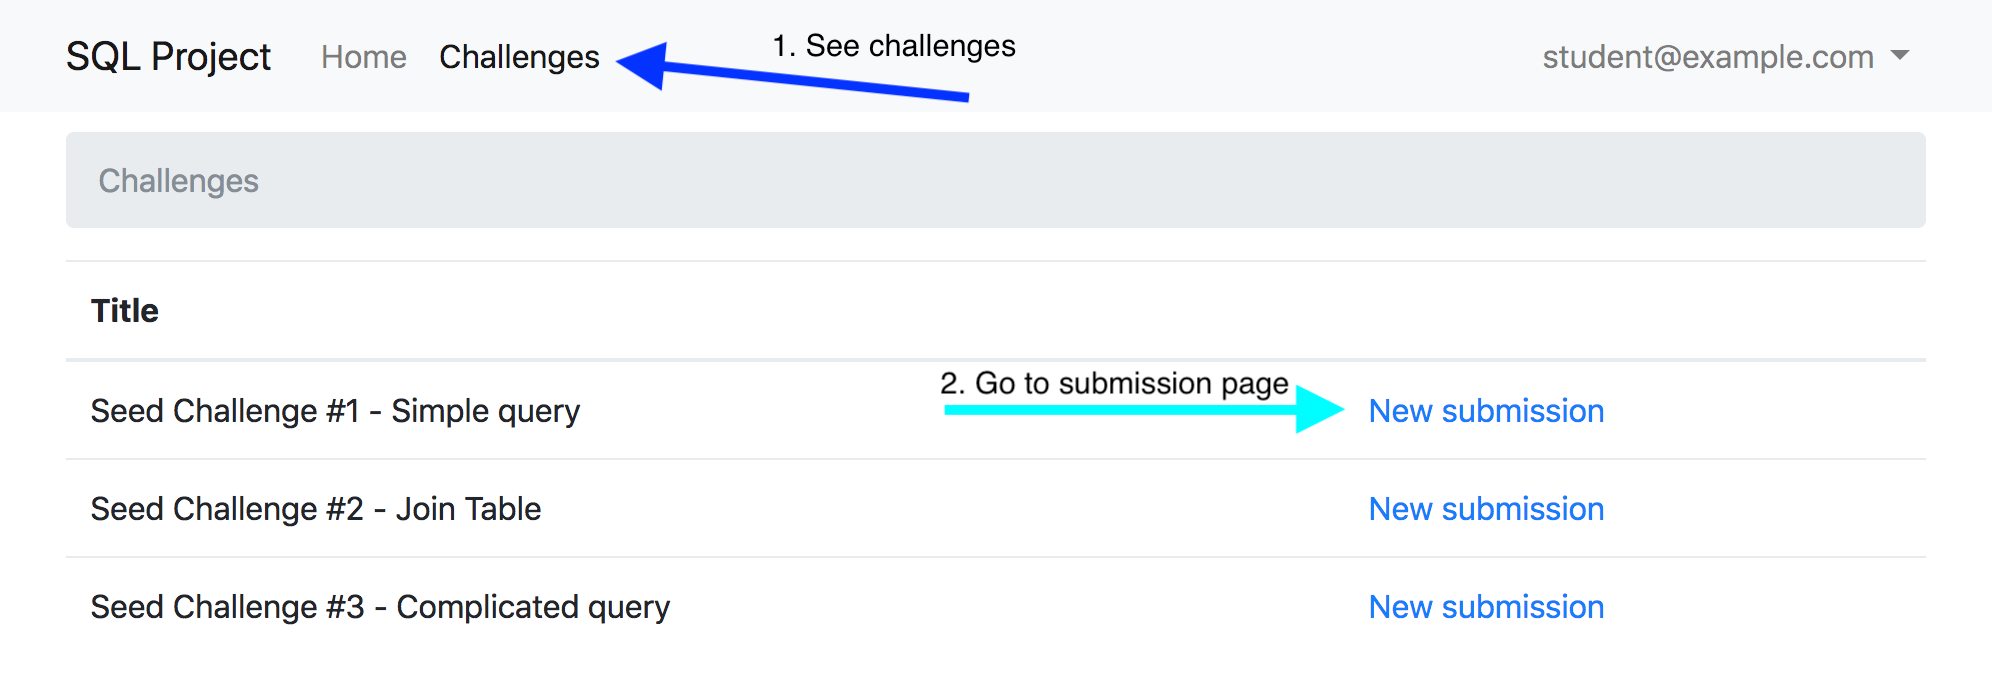
\includegraphics[width=\textwidth/4*3]{Appendices/challengeinde.png}
    \caption{Going to new submission page}
    \label{fig:app:new_submission}
\end{figure}

Once the user gets to that page, he will be able to see the schema of the database, both in the SQL form and in a tabular form. Here he can type the solution to the query. Figure \ref{fig:app:submit} presents this screen.

\begin{figure}[ht]
    \centering
    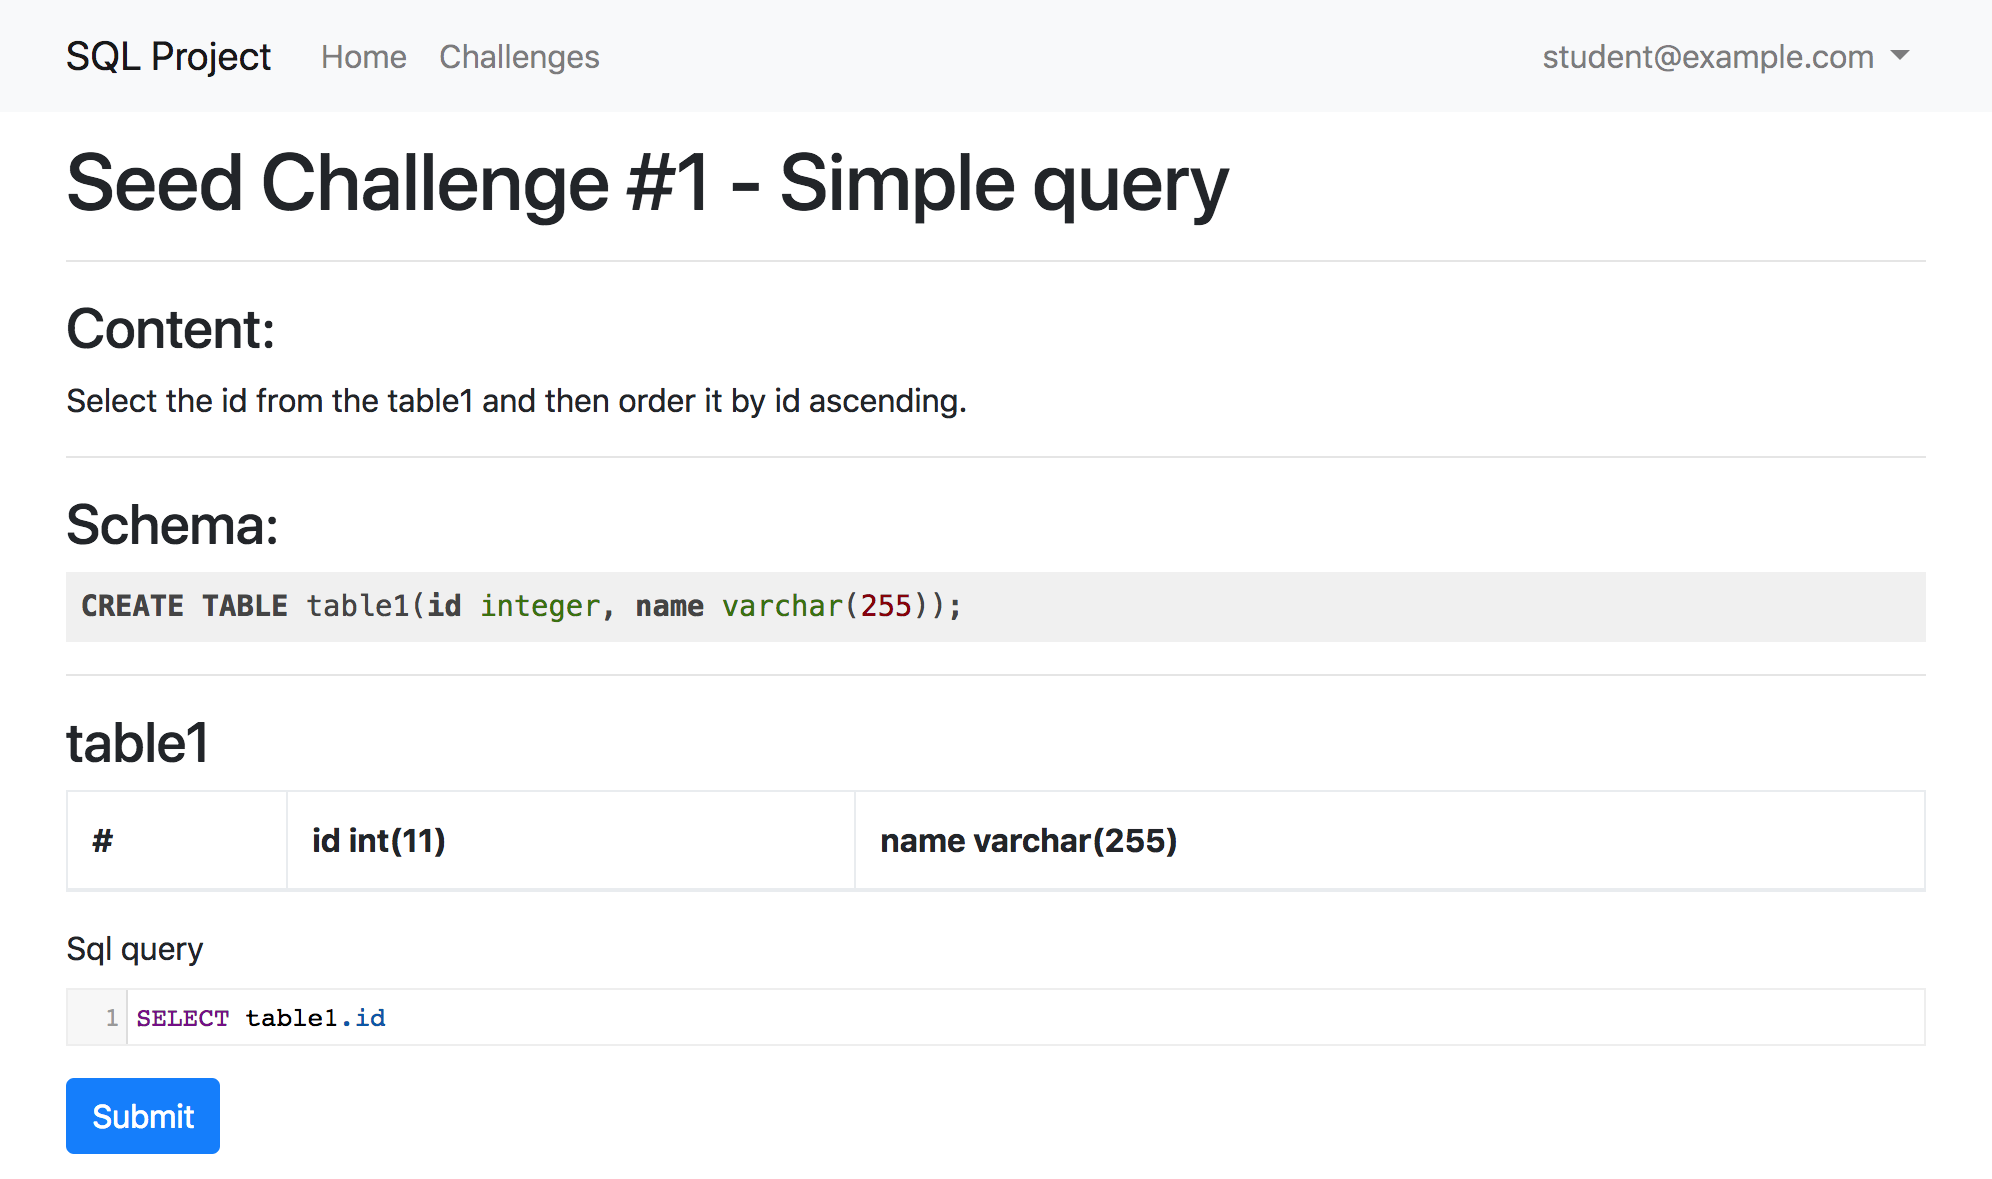
\includegraphics[width=\textwidth/4*3]{Appendices/submit.png}
    \caption{Submit solution page}
    \label{fig:app:submit}
\end{figure}

By clicking the Submit button on the page, the student will be able to see the results of the submission. If the query submitted has SQL errors, the user will see the errors on the same page (example in figure \ref{fig:app:submit_errors}.

\begin{figure}
    \centering
    
\includegraphics[width=\textwidth/4*3]{Appendices/submit_errors.png}
    \caption{Submit errors}
    \label{fig:app:submit_errors}
\end{figure}

If the compilation is successful, the user will either see a success message if the query is correct (figure \ref{fig:app:submit_correct}), or a hint if it's incorrect (figure \ref{fig:app:submit_incorrect}).

\begin{figure}[H]
    \centering
    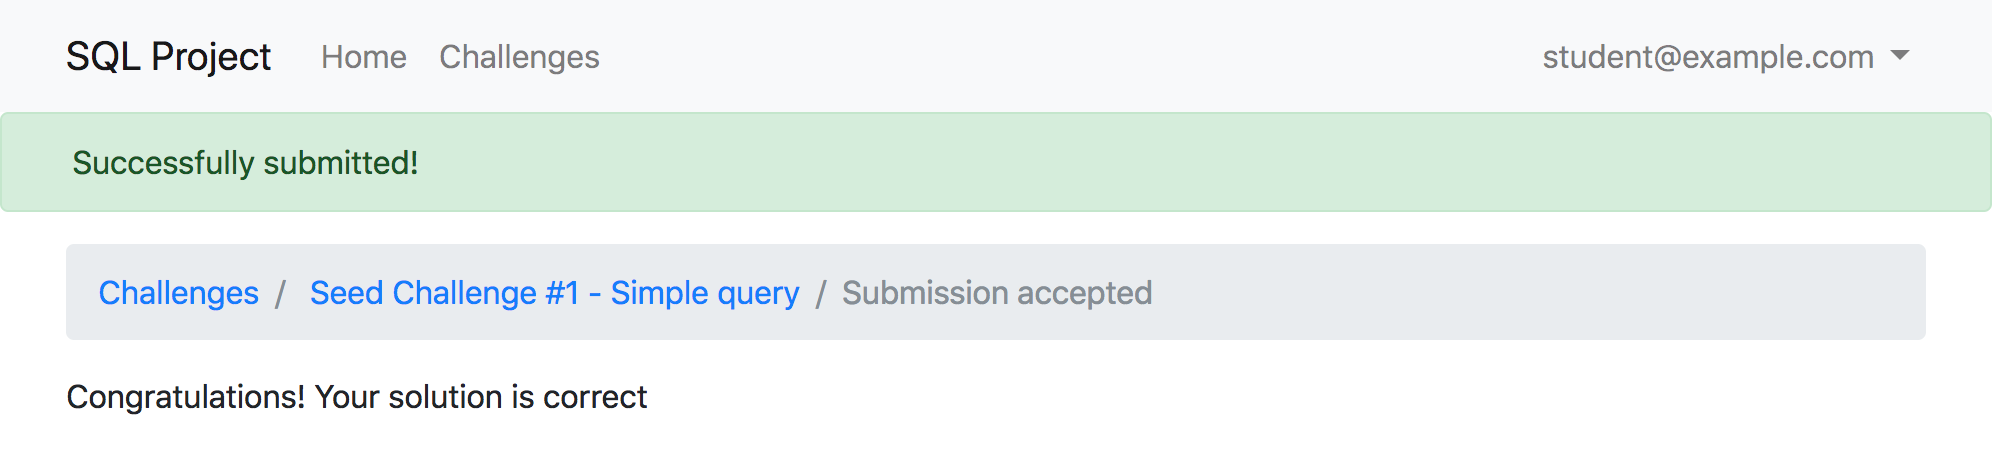
\includegraphics[width=\textwidth/4*3]{Appendices/submit_correct.png}
    \caption{Submission message for correct query}
    \label{fig:app:submit_correct}
\end{figure}

\begin{figure}[H]
    \centering
    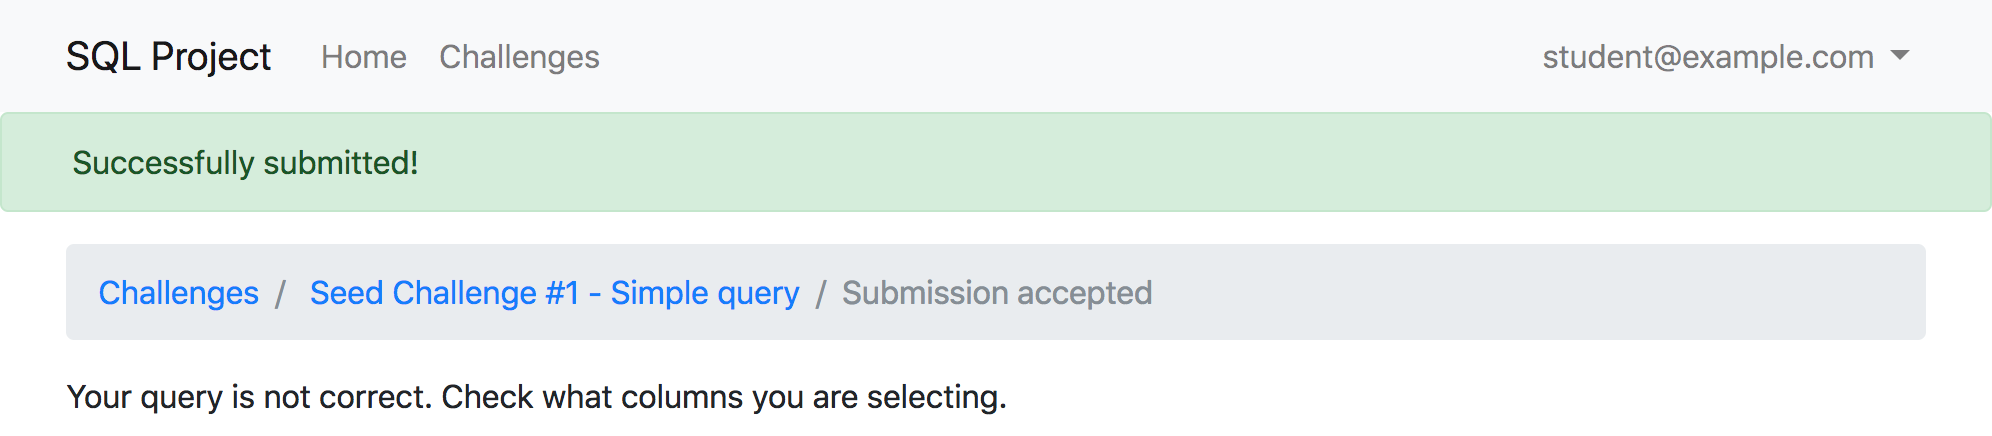
\includegraphics[width=\textwidth/4*3]{Appendices/submit_hint.png}
    \caption{Submission message for correct query}
    \label{fig:app:submit_incorrect}
\end{figure}

\section{Submissions: instructor's view}

To view student's submissions for a challenge, the instructor must click the link "View submissions" from the challenge page (presented in \ref{fig:app:challengeadmin}). The submissions page will include all submissions for a challenge. The page is presented in figure \ref{fig:app:submissions}.

\begin{figure}[ht]
    \centering
    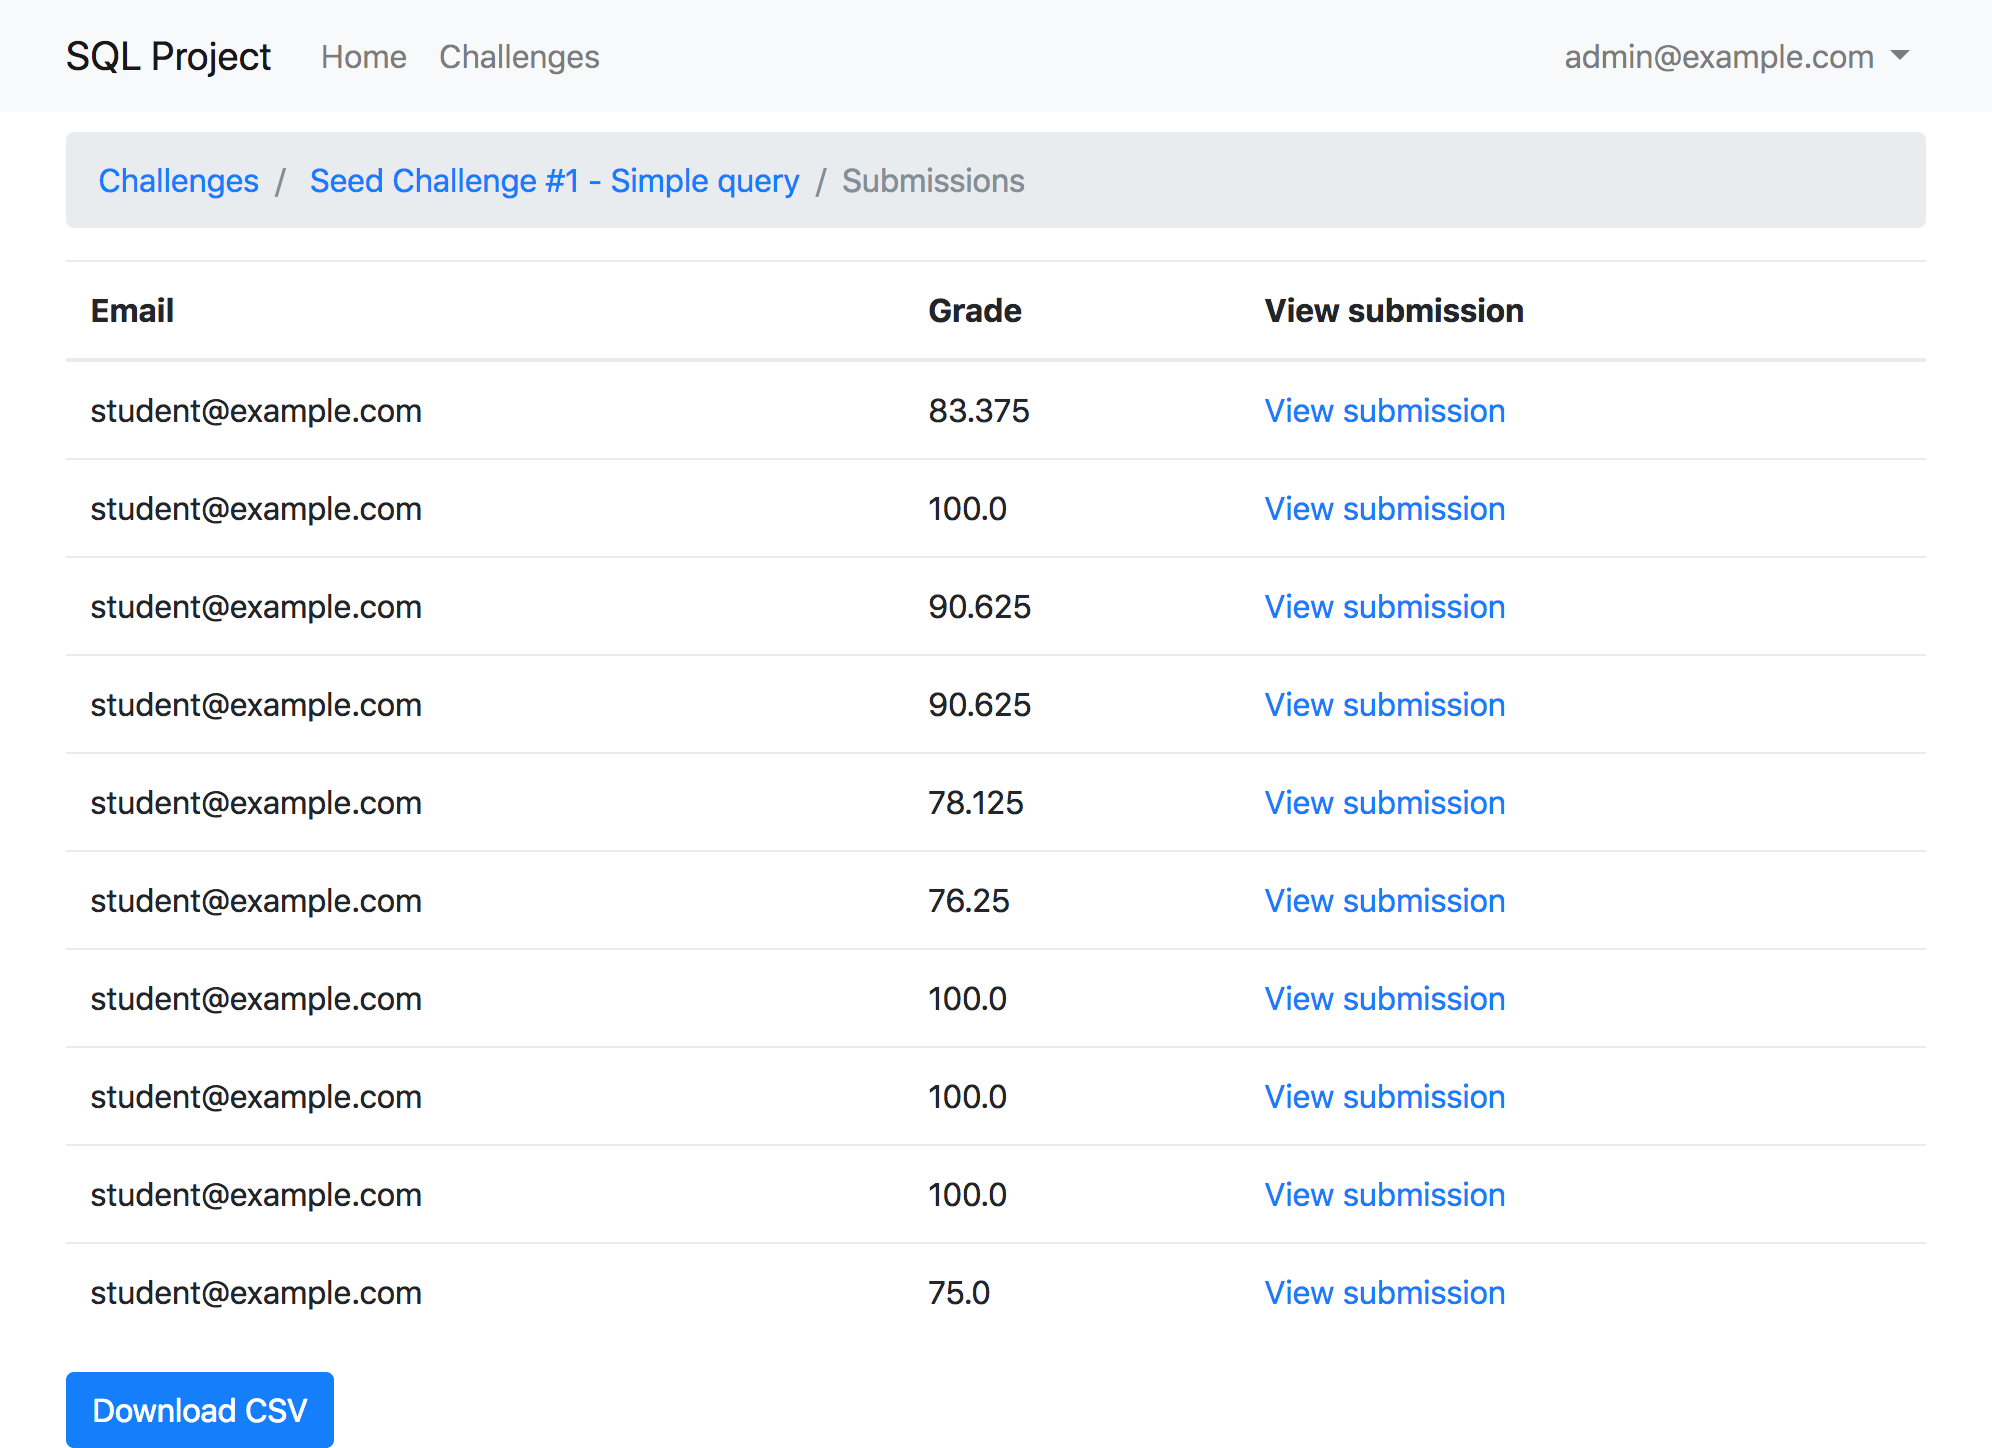
\includegraphics[width=\textwidth/4*3]{Appendices/submissions.png}
    \caption{Submissions for a challenge}
    \label{fig:app:challengeadmin}
\end{figure}

At the bottom of the page there is a Download CSV link that will download a CSV containing the best result for each student.

A instructor can see more details about a submission by clicking the View submission link. The new page will include all details about a submission. An example of such a page is included in figure \ref{fig:app:submission_report}.

\begin{figure}
    \centering
    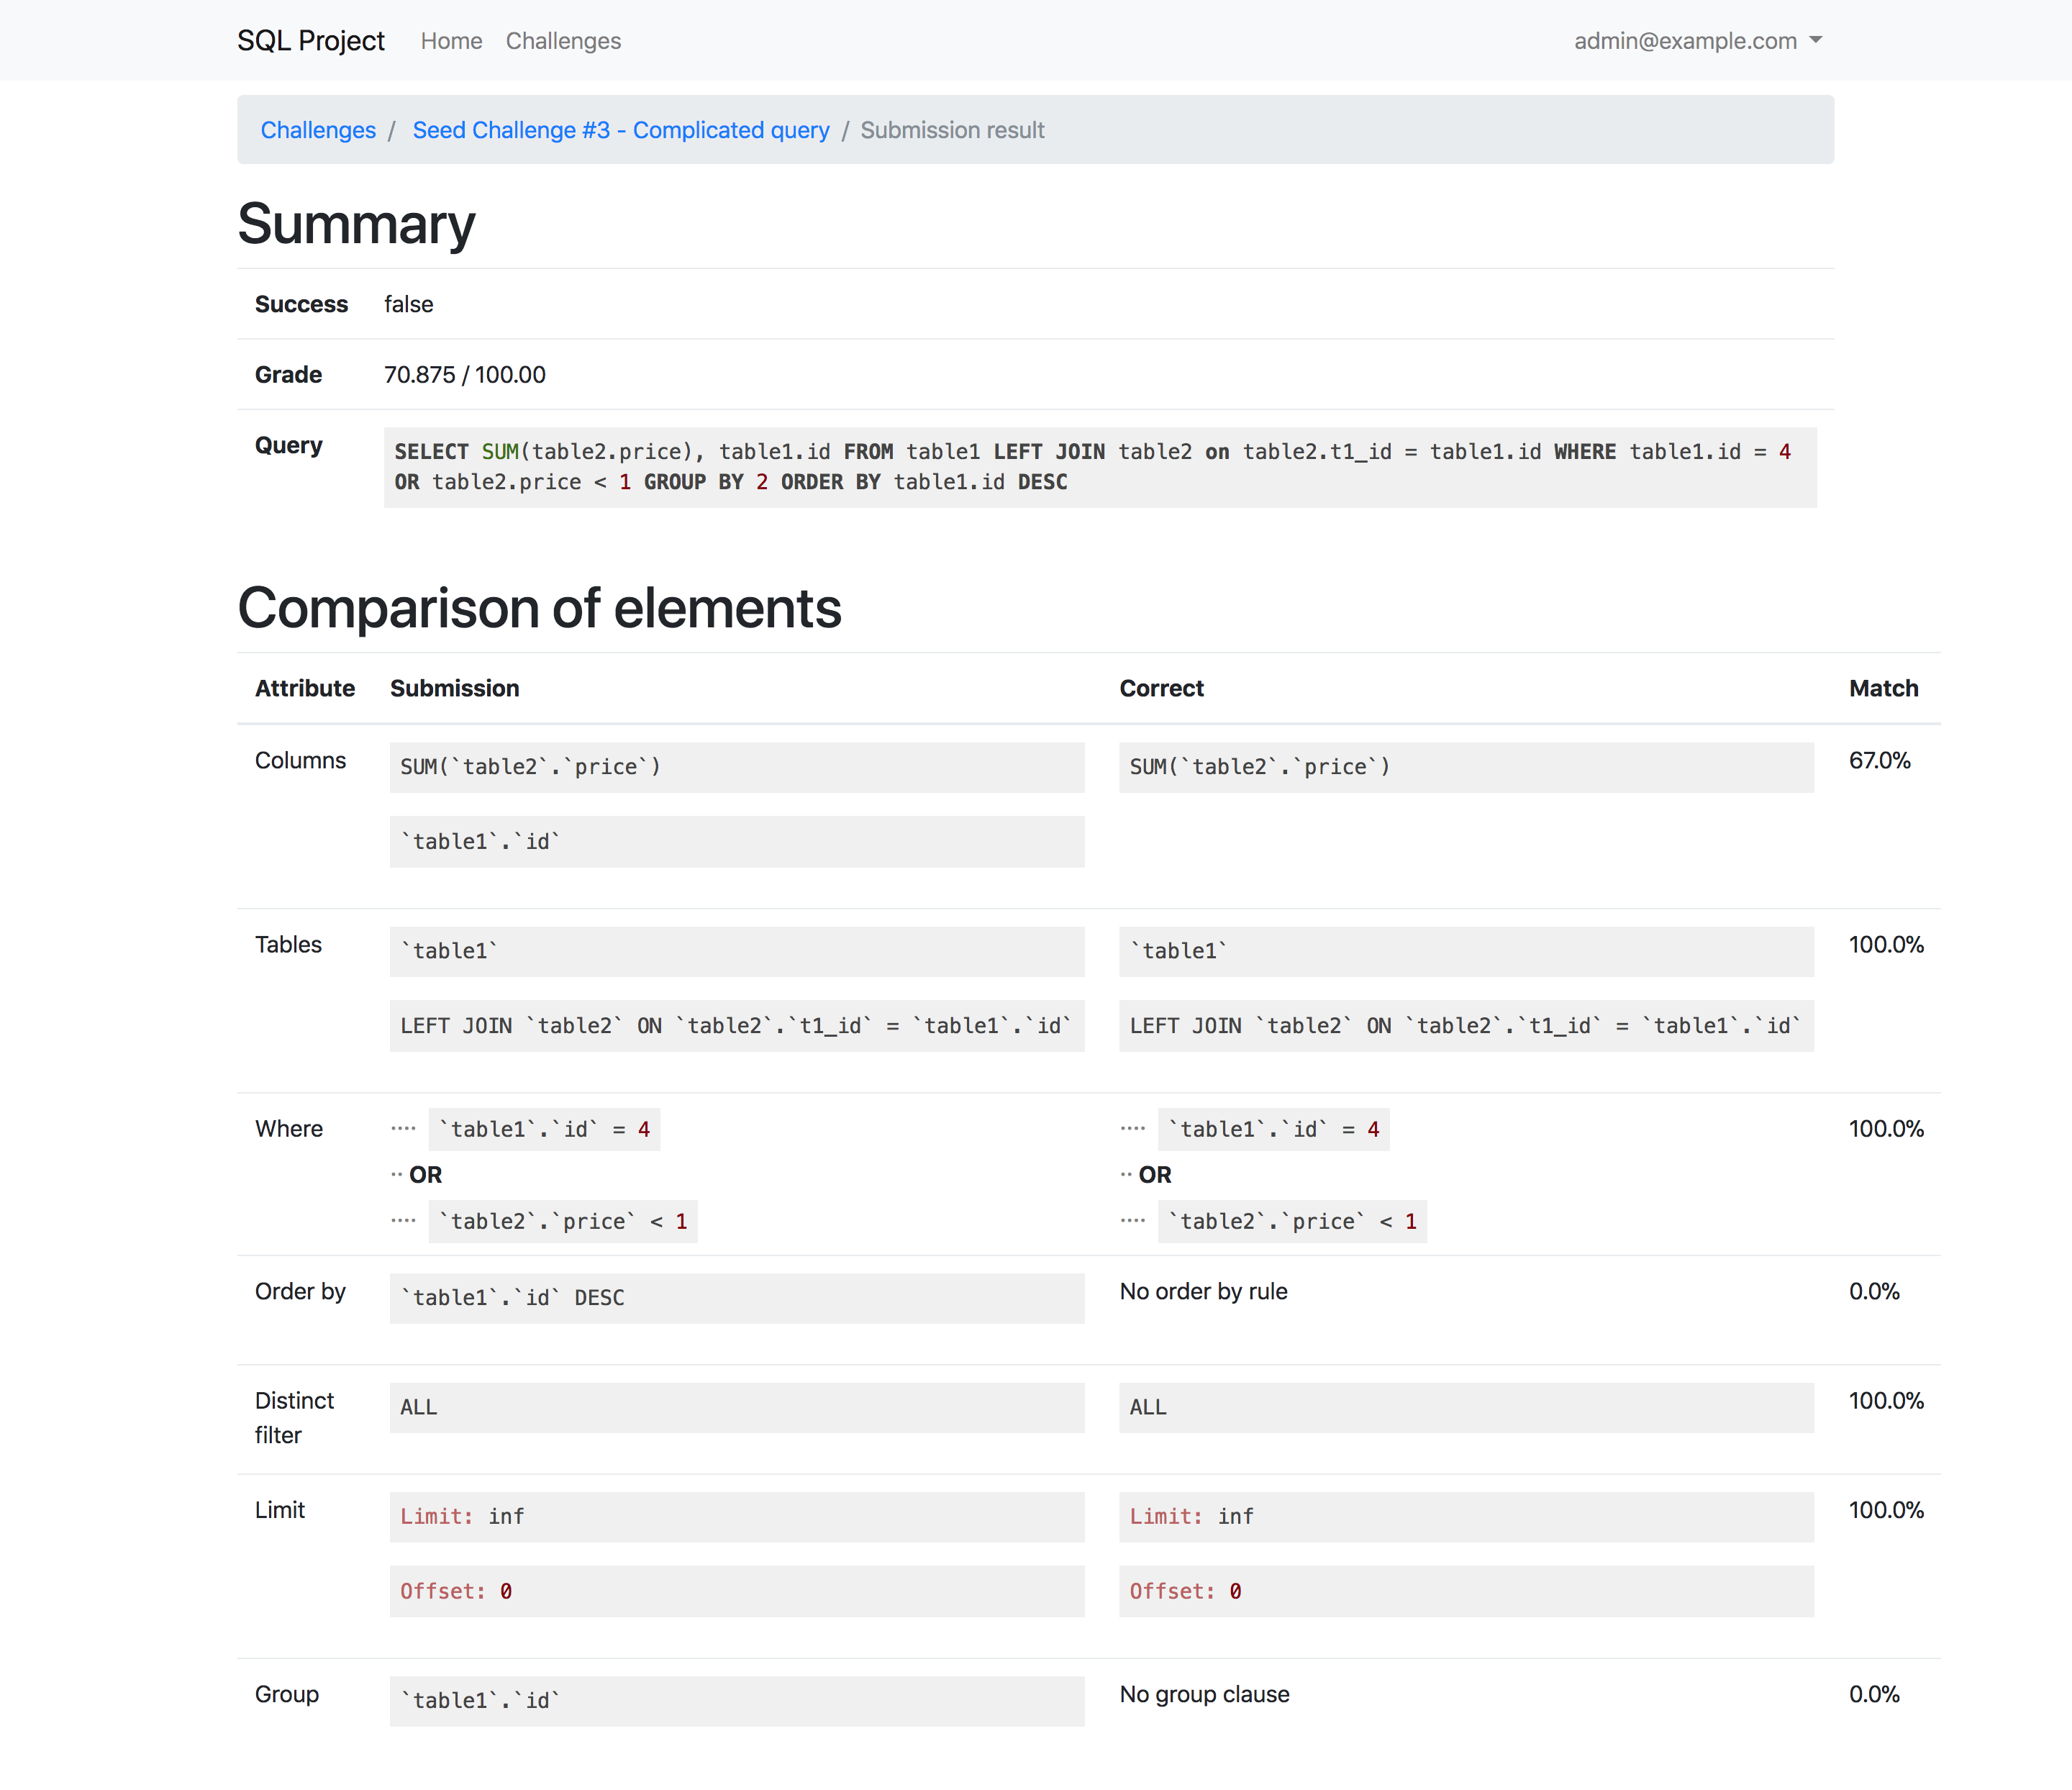
\includegraphics[width=\textwidth/4*3]{Appendices/submission_report.png}
    \caption{Caption}
    \label{fig:app:submission_report}
\end{figure}
% \chapter{Source Code}
\section{Instructions}
Complete source code listings must be submitted as an appendix to the report. The project source codes are usually spread out over several files/units. You should try to help the reader to navigate through your source code by providing a ``table of contents'' (titles of these files/units and one line descriptions). The first page of the program listings folder must contain the following statement certifying the work as your own: ``I verify that I am the sole author of the programs contained in this folder, except where explicitly stated to the contrary''. Your (typed) signature and the date should follow this statement.

All work on programs must stop once the code is submitted to KEATS. You are required to keep safely several copies of this version of the program and you must use one of these copies in the project examination. Your examiners may ask to see the last-modified dates of your program files, and may ask you to demonstrate that the program files you use in the project examination are identical to the program files you have uploaded to KEATS. Any attempt to demonstrate code that is not included in your submitted source listings is an attempt to cheat; any such attempt will be reported to the KCL Misconduct Committee.

\textbf{You may find it easier to firstly generate a PDF of your source code using a text editor and then merge it to the end of your report. There are many free tools available that allow you to merge PDF files.}


\end{document}
